\section{Results}
First, we use synthetic data to show that $\texttt{inlabru}$ produces restults that are sufficiently similar to the one produced by more traditional MCMC approaches. For a fair comparison between the $\texttt{INLA}$ framework and state-of-the-art MCMC methods, we compare results of Bayesian inference using $\texttt{inlabru}$ to results using inference from the STAN methodology. The STAN methodology is an implementation of a Hamiltonian Monte Carlo approach, and is described more closely in Section \ref{sec:stan}. We use the $\texttt{R}$-library $\texttt{rstan}$ to do inference with STAN. 

\subsection{STAN: Hamiltonian Monte Carlo}
\label{sec:stan}
STAN is a method for Bayesian inference using a Hamiltonian Monte Carlo approach. It was proposed by ... and has since its introduction gained popularity for its computational power compared to traditional MCMC approaches. bla bla ikke ferdig!!!

\newpage
\subsection{Preliminary Analysis With Synthetic Data}
\label{sec:synthetic-data}
To demonstrate that the \inlabru method is able to correclty identify the underlying age and period effects when we apply the LC-model to mortality data, we compare results produced using \inlabru to results produced using \stan. We define some values for the model components in the LC-model, and use these to sample values for synthetic mortality. We display the synthetic random effects, with their associated hyperparameters together with the estimated random effects as estimated by \inlabru and \stan. 

% v10.3 - predictor
\begin{figure}
    \centering
    \textbf{v10.3: Estimated predictor}
    \begin{subfigure}[b]{.85\linewidth}
        \includegraphics[width=\linewidth]{Master Thesis Code/Scripts/Synthetic data/Output/Figures/v10_3_rw2/eta_x_comparison.pdf}
        \caption{The predictor \etaxt displayed as a function of calendar year, for each age group. }
        \label{fig:eta-v10_3-x}
    \end{subfigure}
    
    \begin{subfigure}[b]{.85\linewidth}
        \includegraphics[width=\linewidth]{Master Thesis Code/Scripts/Synthetic data/Output/Figures/v10_3_rw2/eta_t_comparison.pdf}
        \caption{The predictor \etaxt displayed as a function of age, for each available calendar year. }
        \label{fig:eta-v10_3-t}
    \end{subfigure}
    \caption{The predictor \etaxt estimated by \inlabru and \stan displayed together with the synthetic value for the predictor \etaxt.}
    \label{fig:eta-v10_3}
\end{figure}

% v10.3 - random effects
\begin{figure}
    \centering
    \textbf{v10.3: Estimated random effects}
    \begin{subfigure}[b]{.85\linewidth}
        \includegraphics[width=\linewidth]{Master Thesis Code/Scripts/Synthetic data/Output/Figures/v10_3_rw2/random_effects_comparison.pdf}
        \caption{Estimated random effects.}
        \label{fig:random-effects-v10-3-re}
    \end{subfigure}
    
    \begin{subfigure}[b]{.85\linewidth}
        \includegraphics[width=\linewidth]{Master Thesis Code/Scripts/Synthetic data/Output/Figures/v10_3_rw2/hypers_comparison.pdf}
        \caption{Estimated hyperparameters}
        \label{fig:random-effects-v10-3-hyper}
    \end{subfigure}
    \caption{The age and period effects as estimated by \inlabru and \stan, together with the synthetic random effects. }
    \label{fig:random-effects-v10-3}
\end{figure}

% v10.3 - trace
\begin{figure}
    \centering
    \textbf{Male stomach cancer: Trace plots from \stan}
    \begin{subfigure}[b]{.45\linewidth}
        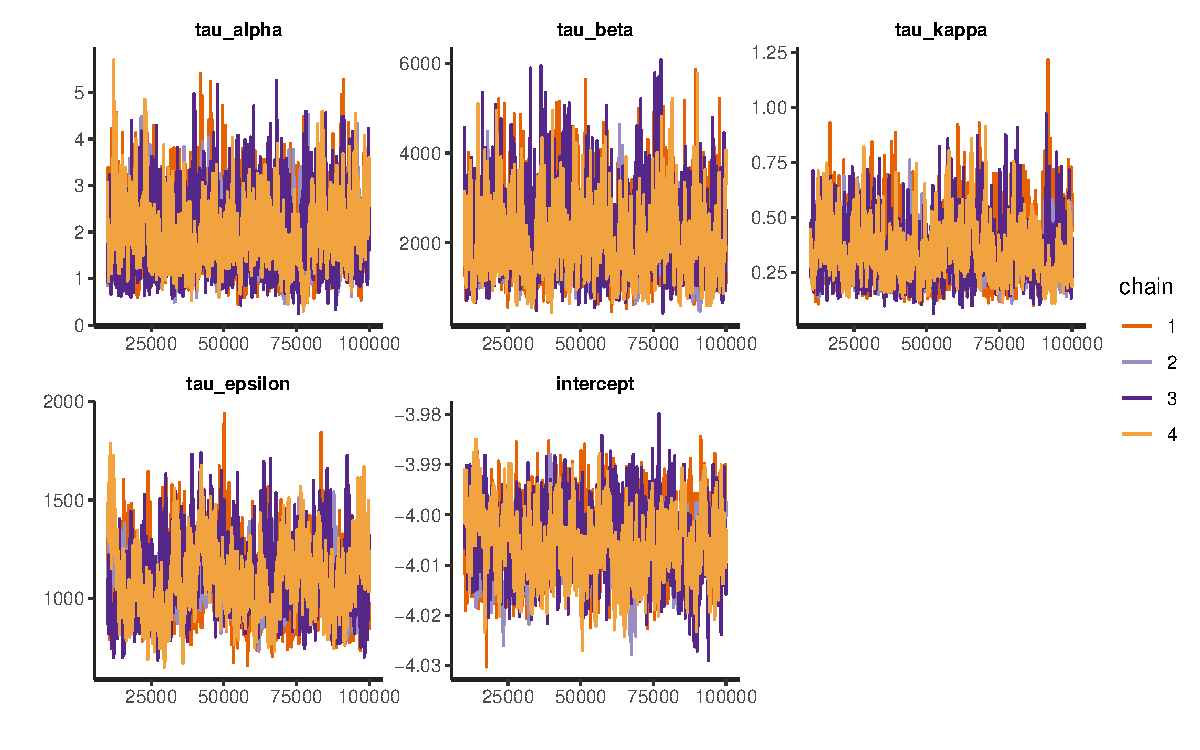
\includegraphics[width=\linewidth]{Master Thesis Code/Scripts/Synthetic data/Stan analyses/v10_3/stan_results/trace_hyperpars.pdf}
        \caption{Trace plots for hyperparameters}
        \label{fig:v10_3-trace-hypers}
    \end{subfigure}
    \begin{subfigure}[b]{.45\linewidth}
        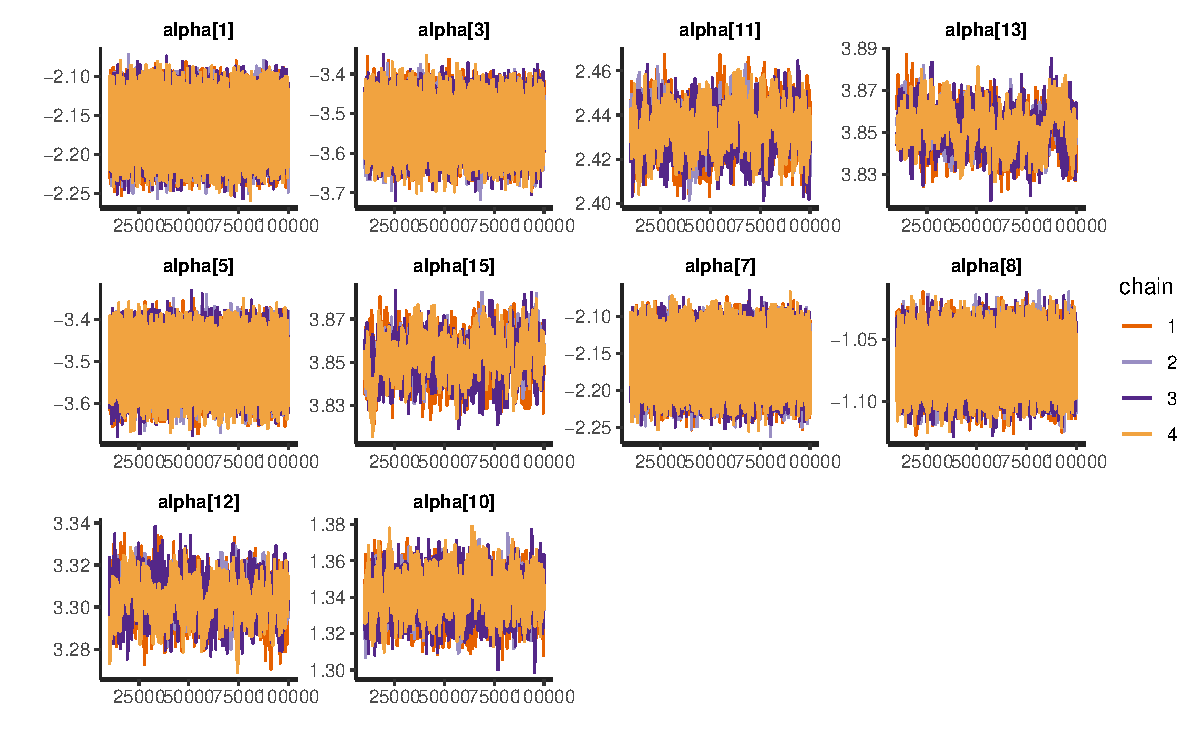
\includegraphics[width=\linewidth]{Master Thesis Code/Scripts/Synthetic data/Stan analyses/v10_3/stan_results/trace_alpha.pdf}
        \caption{Trace plots for selected values of $\alpha_x$}
        \label{fig:v10_3-trace-alpha}
    \end{subfigure}
    
    \begin{subfigure}[b]{.45\linewidth}
        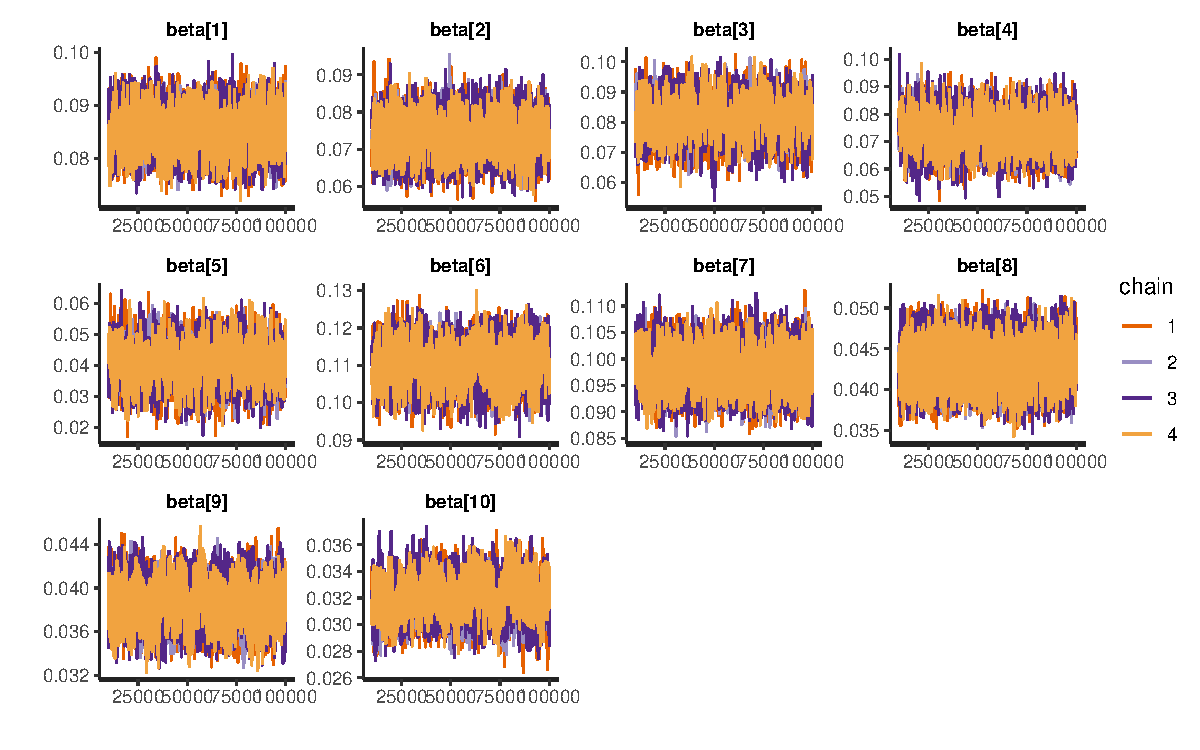
\includegraphics[width=\linewidth]{Master Thesis Code/Scripts/Synthetic data/Stan analyses/v10_3/stan_results/trace_beta.pdf}
        \caption{Trace plots for selected values of $\beta_x$}
        \label{fig:v10_3-trace-beta}
    \end{subfigure}
    \begin{subfigure}[b]{.45\linewidth}
        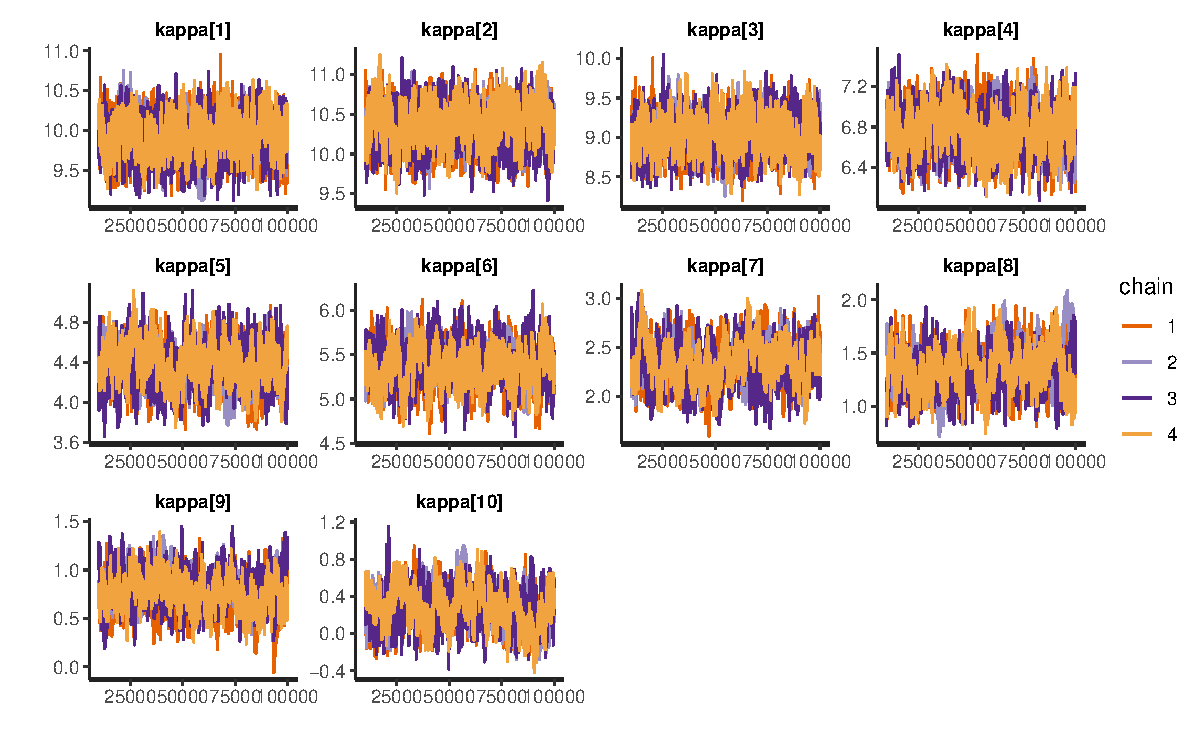
\includegraphics[width=\linewidth]{Master Thesis Code/Scripts/Synthetic data/Stan analyses/v10_3/stan_results/trace_kappa.pdf}
        \caption{Trace plots for selected values of $\kappa_t$}
        \label{fig:v10_3-trace-kappa}
    \end{subfigure}
    \caption{Trace plots from inference using \stan for configuration v10.3. }
    \label{fig:v10_3-trace}
\end{figure}

% v12.3 - predictor
\begin{figure}
    \centering
    \textbf{v12.3: Estimated predictor}
    \begin{subfigure}[b]{.85\linewidth}
        \includegraphics[width=\linewidth]{Master Thesis Code/Scripts/Synthetic data/Output/Figures/v12_3_rw2/eta_x_comparison.pdf}
        \caption{The predictor \etaxt displayed as a function of calendar year, for each age group. }
        \label{fig:eta-v12_3-x}
    \end{subfigure}
    
    \begin{subfigure}[b]{.85\linewidth}
        \includegraphics[width=\linewidth]{Master Thesis Code/Scripts/Synthetic data/Output/Figures/v12_3_rw2/eta_t_comparison.pdf}
        \caption{The predictor \etaxt displayed as a function of age, for each available calendar year. }
        \label{fig:eta-v12_3-t}
    \end{subfigure}
    \caption{The predictor \etaxt estimated by \inlabru and \stan displayed together with the synthetic value for the predictor \etaxt.}
    \label{fig:eta-v12_3}
\end{figure}

% v12.3 - Random effects
\begin{figure}
    \centering
    \textbf{v12.3: Estimated random effects}
    \begin{subfigure}[b]{.85\linewidth}
        \includegraphics[width=\linewidth]{Master Thesis Code/Scripts/Synthetic data/Output/Figures/v12_3_rw2/random_effects_comparison.pdf}
        \caption{Estimated random effects.}
        \label{fig:random-effects-v12-3-re}
    \end{subfigure}
    
    \begin{subfigure}[b]{.85\linewidth}
        \includegraphics[width=\linewidth]{Master Thesis Code/Scripts/Synthetic data/Output/Figures/v12_3_rw2/hypers_comparison.pdf}
        \caption{Estimated hyperparameters}
        \label{fig:random-effects-v12-3-hyper}
    \end{subfigure}
    \caption{The age and period effects as estimated by \inlabru and \stan, together with the synthetic random effects. }
    \label{fig:random-effects-v12-3}
\end{figure}

% v12.3 - trace plots
\begin{figure}
    \centering
    \textbf{Male stomach cancer: Trace plots from \stan}
    \begin{subfigure}[b]{.45\linewidth}
        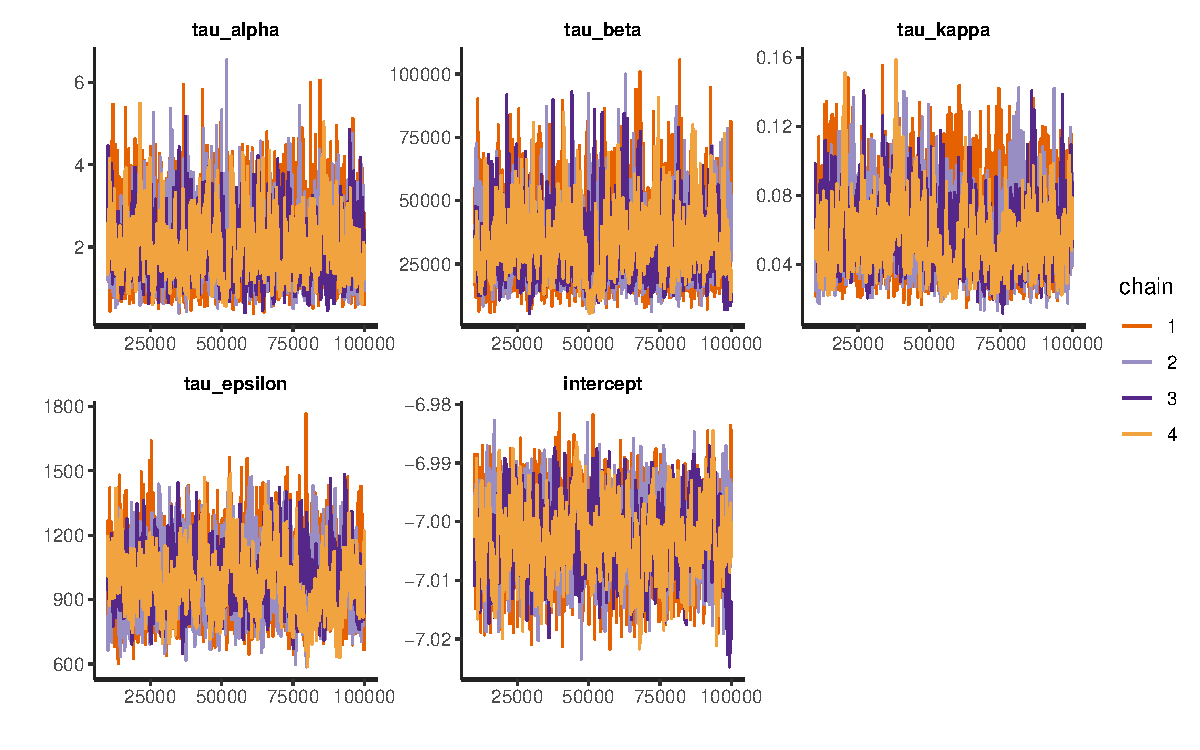
\includegraphics[width=\linewidth]{Master Thesis Code/Scripts/Synthetic data/Stan analyses/v12_3/stan_results/trace_hyperpars.pdf}
        \caption{Trace plots for hyperparameters}
        \label{fig:v12_3-trace-hypers}
    \end{subfigure}
    \begin{subfigure}[b]{.45\linewidth}
        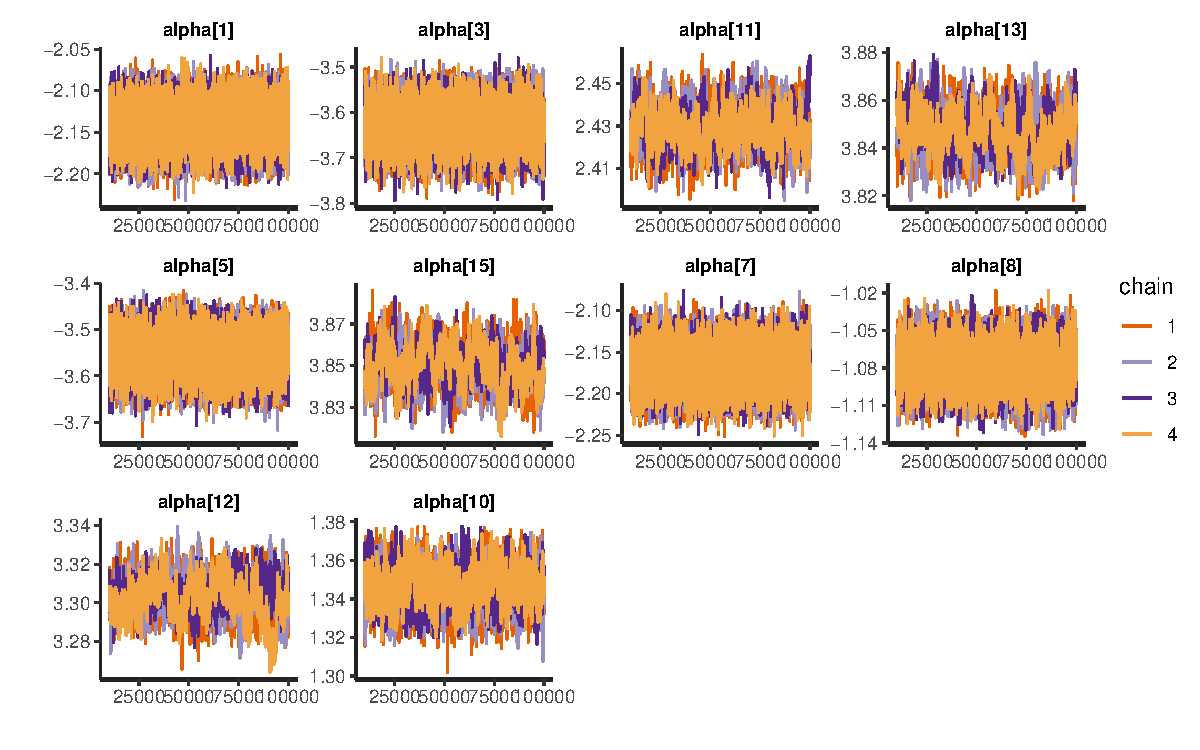
\includegraphics[width=\linewidth]{Master Thesis Code/Scripts/Synthetic data/Stan analyses/v12_3/stan_results/trace_alpha.pdf}
        \caption{Trace plots for selected values of $\alpha_x$}
        \label{fig:v12_3-trace-alpha}
    \end{subfigure}
    
    \begin{subfigure}[b]{.45\linewidth}
        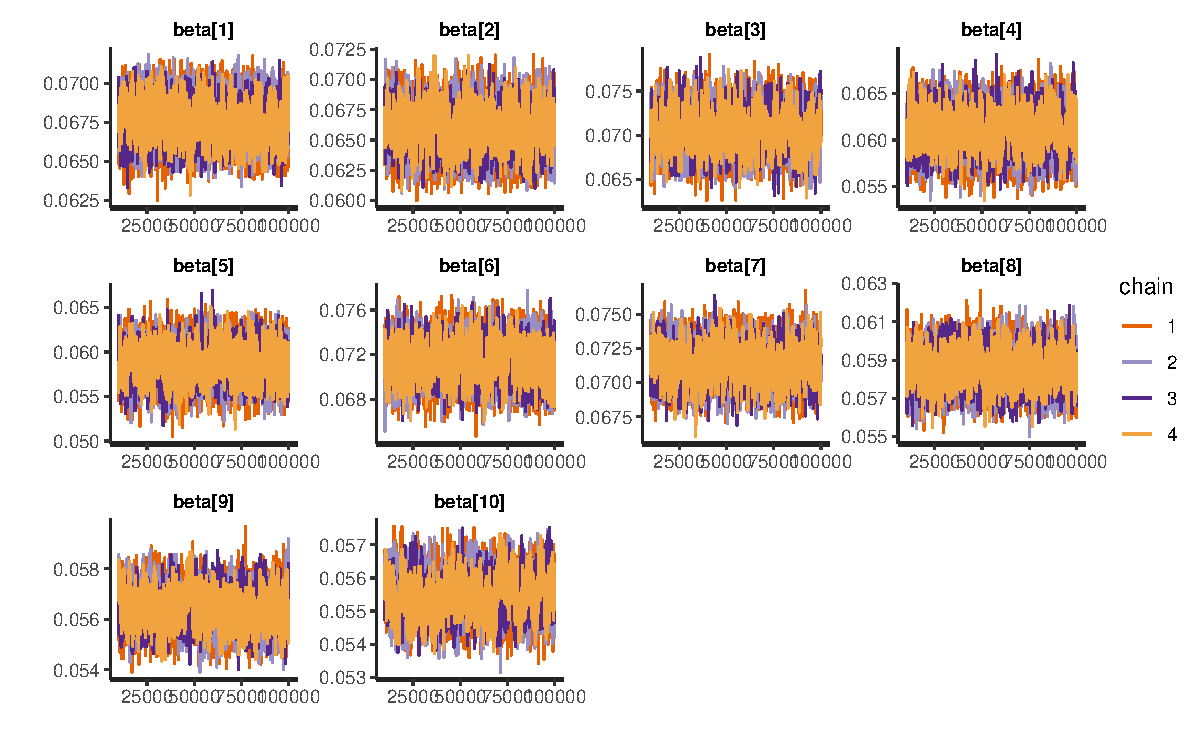
\includegraphics[width=\linewidth]{Master Thesis Code/Scripts/Synthetic data/Stan analyses/v12_3/stan_results/trace_beta.pdf}
        \caption{Trace plots for selected values of $\beta_x$}
        \label{fig:v12_3-trace-beta}
    \end{subfigure}
    \begin{subfigure}[b]{.45\linewidth}
        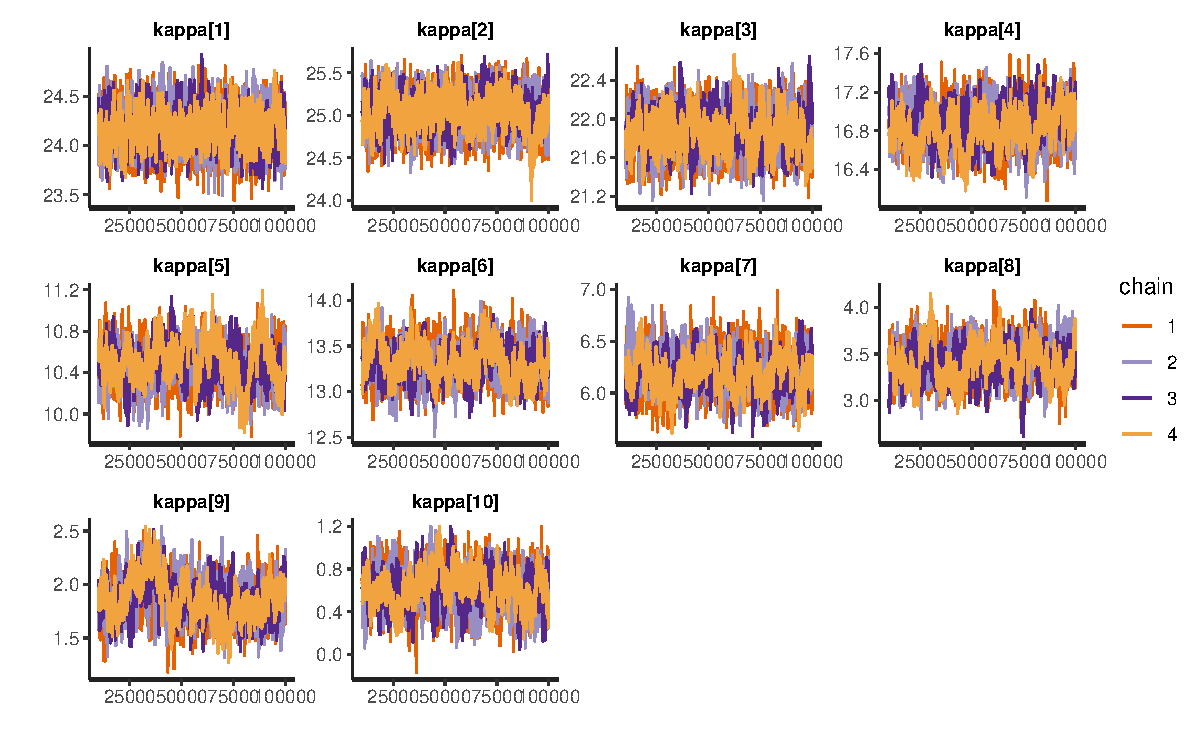
\includegraphics[width=\linewidth]{Master Thesis Code/Scripts/Synthetic data/Stan analyses/v12_3/stan_results/trace_kappa.pdf}
        \caption{Trace plots for selected values of $\kappa_t$}
        \label{fig:v12_3-trace-kappa}
    \end{subfigure}
    \caption{Trace plots from inference using \stan for configuration v12.3. }
    \label{fig:v12_3-trace}
\end{figure}

% Synthetic male stomach - predictor
\begin{figure}
    \centering
    \textbf{Synthetic male stomach: Estimated predictor}
    \begin{subfigure}[b]{.85\linewidth}
        \includegraphics[width=\linewidth]{Master Thesis Code/Scripts/Synthetic data/Output/Figures/synthetic_male_stomach_lc/eta_x_comparison.pdf}
        \caption{The predictor \etaxt displayed as a function of calendar year, for each age group. }
        \label{fig:eta-synthetic_male_stomach_lc-x}
    \end{subfigure}
    
    \begin{subfigure}[b]{.85\linewidth}
        \includegraphics[width=\linewidth]{Master Thesis Code/Scripts/Synthetic data/Output/Figures/synthetic_male_stomach_lc/eta_t_comparison.pdf}
        \caption{The predictor \etaxt displayed as a function of age, for each available calendar year. }
        \label{fig:eta-synthetic_male_stomach_lc-t}
    \end{subfigure}
    \caption{The predictor \etaxt estimated by \inlabru and \stan displayed together with the synthetic value for the predictor \etaxt.}
    \label{fig:eta-synthetic_male_stomach_lc}
\end{figure}

% Synthetic male stomach - random effects 
\begin{figure}
    \centering
    \textbf{Synthetic male stomach: Estimated random effects}
    \begin{subfigure}[b]{.85\linewidth}
        \includegraphics[width=\linewidth]{Master Thesis Code/Scripts/Synthetic data/Output/Figures/synthetic_male_stomach_lc/random_effects_comparison.pdf}
        \caption{Estimated random effects.}
        \label{fig:random-effects-synthetic_male_stomach_lc-re}
    \end{subfigure}
    
    \begin{subfigure}[b]{.85\linewidth}
        \includegraphics[width=\linewidth]{Master Thesis Code/Scripts/Synthetic data/Output/Figures/synthetic_male_stomach_lc/hypers_comparison.pdf}
        \caption{Estimated hyperparameters}
        \label{fig:random-effects-synthetic_male_stomach_lc-hyper}
    \end{subfigure}
    \caption{The age and period effects as estimated by \inlabru and \stan, together with the synthetic random effects. }
    \label{fig:random-effects-synthetic_male_stomach_lc}
\end{figure}

% Synthetic male stomach - trace plots 
\begin{figure}
    \centering
    \textbf{Male stomach cancer: Trace plots from \stan}
    \begin{subfigure}[b]{.45\linewidth}
        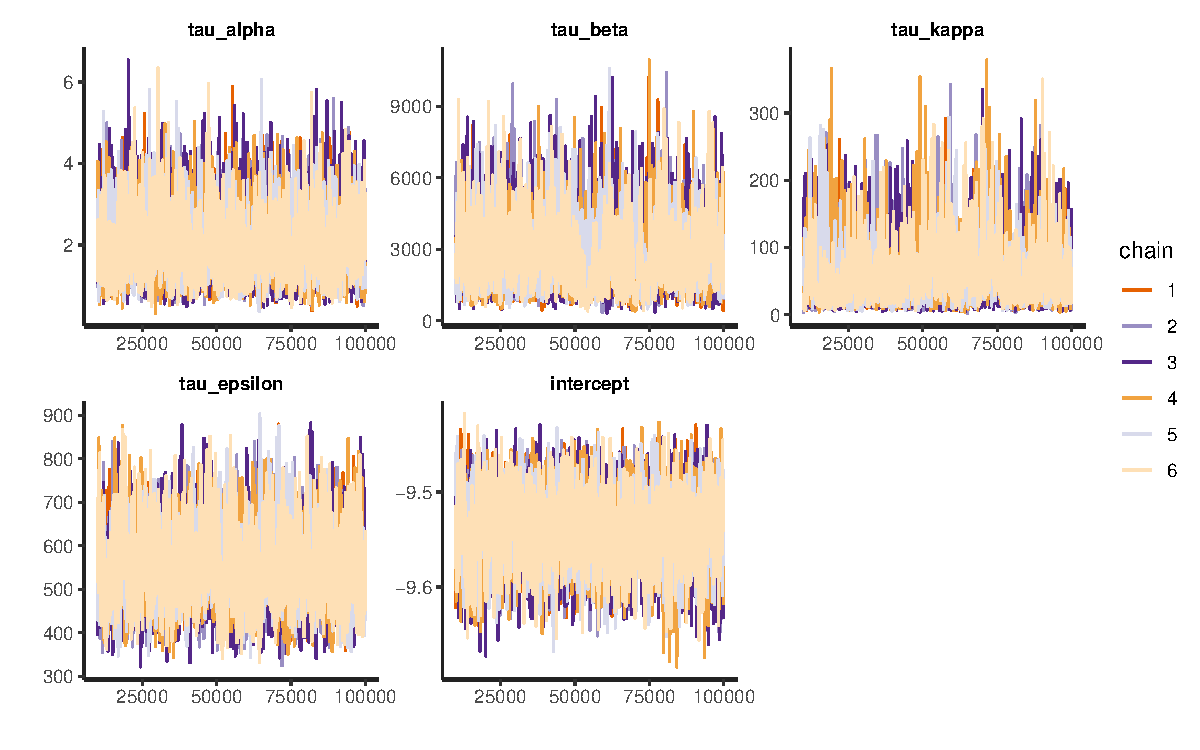
\includegraphics[width=\linewidth]{Master Thesis Code/Scripts/Synthetic data/Stan analyses/synthetic_male_stomach_lc/stan_results/trace_hyperpars.pdf}
        \caption{Trace plots for hyperparameters}
        \label{fig:synthetic_male_stomach_lc-trace-hypers}
    \end{subfigure}
    \begin{subfigure}[b]{.45\linewidth}
        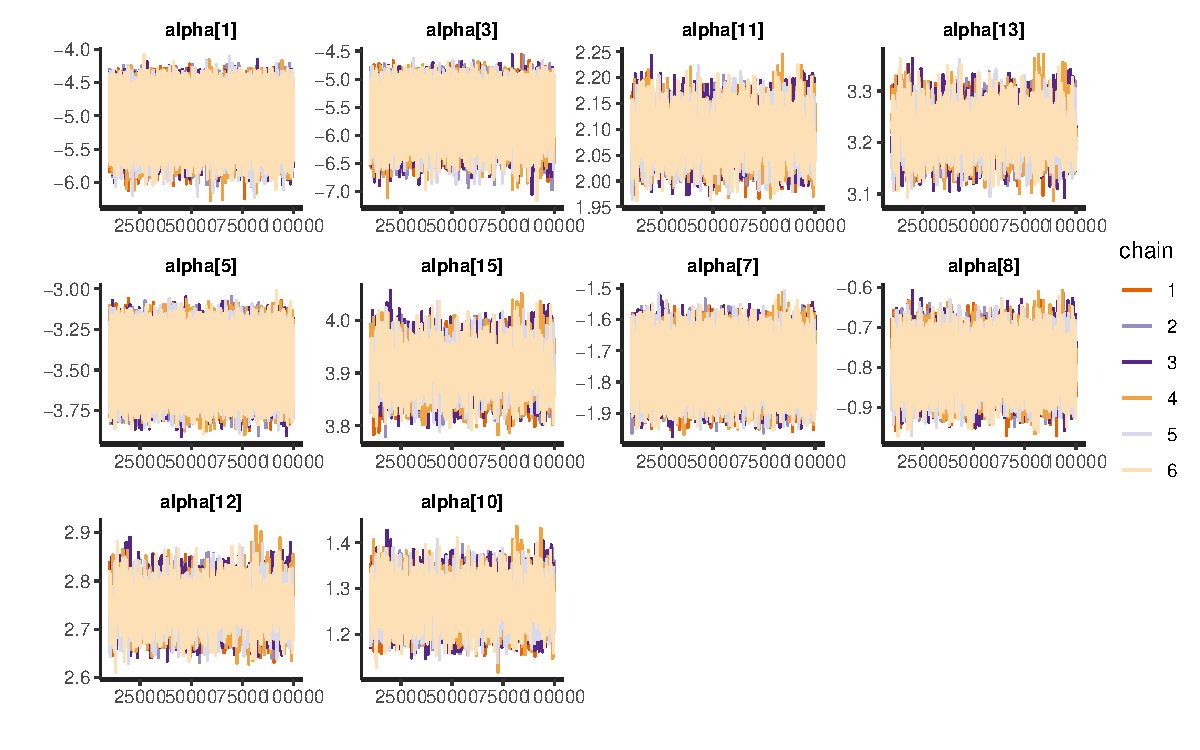
\includegraphics[width=\linewidth]{Master Thesis Code/Scripts/Synthetic data/Stan analyses/synthetic_male_stomach_lc/stan_results/trace_alpha.pdf}
        \caption{Trace plots for selected values of $\alpha_x$}
        \label{fig:synthetic_male_stomach_lc-trace-alpha}
    \end{subfigure}
    
    \begin{subfigure}[b]{.45\linewidth}
        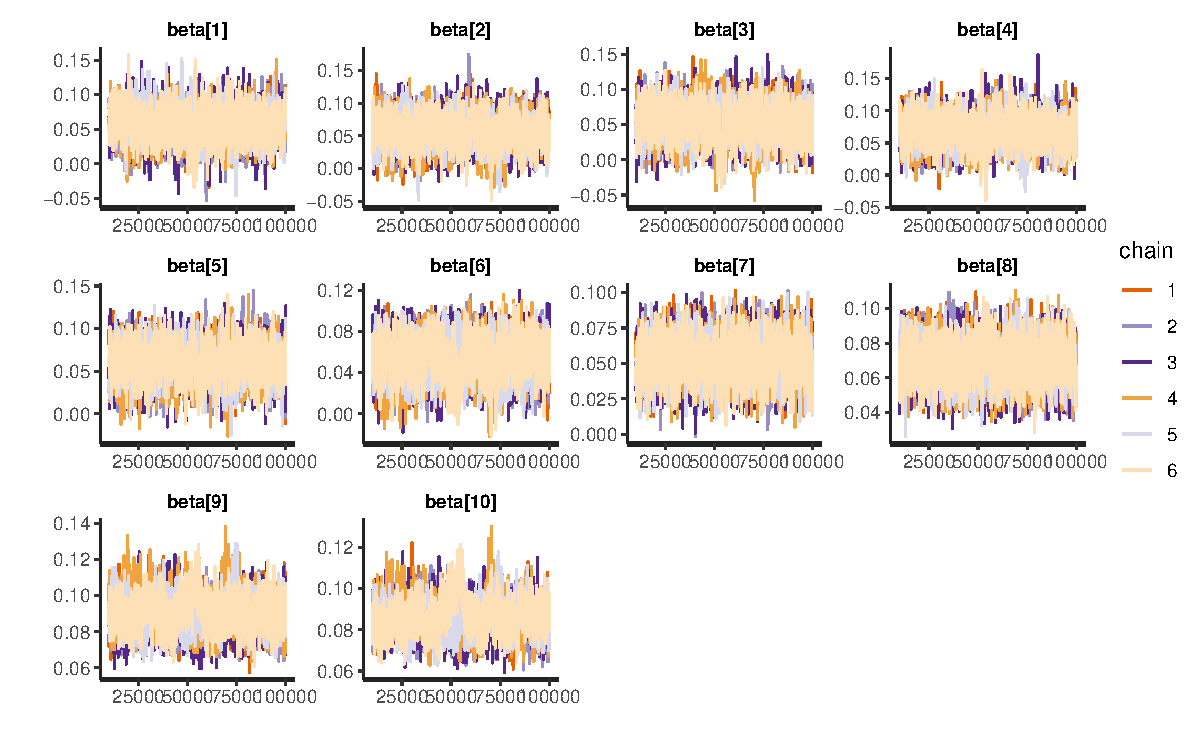
\includegraphics[width=\linewidth]{Master Thesis Code/Scripts/Synthetic data/Stan analyses/synthetic_male_stomach_lc/stan_results/trace_beta.pdf}
        \caption{Trace plots for selected values of $\beta_x$}
        \label{fig:synthetic_male_stomach_lc-trace-beta}
    \end{subfigure}
    \begin{subfigure}[b]{.45\linewidth}
        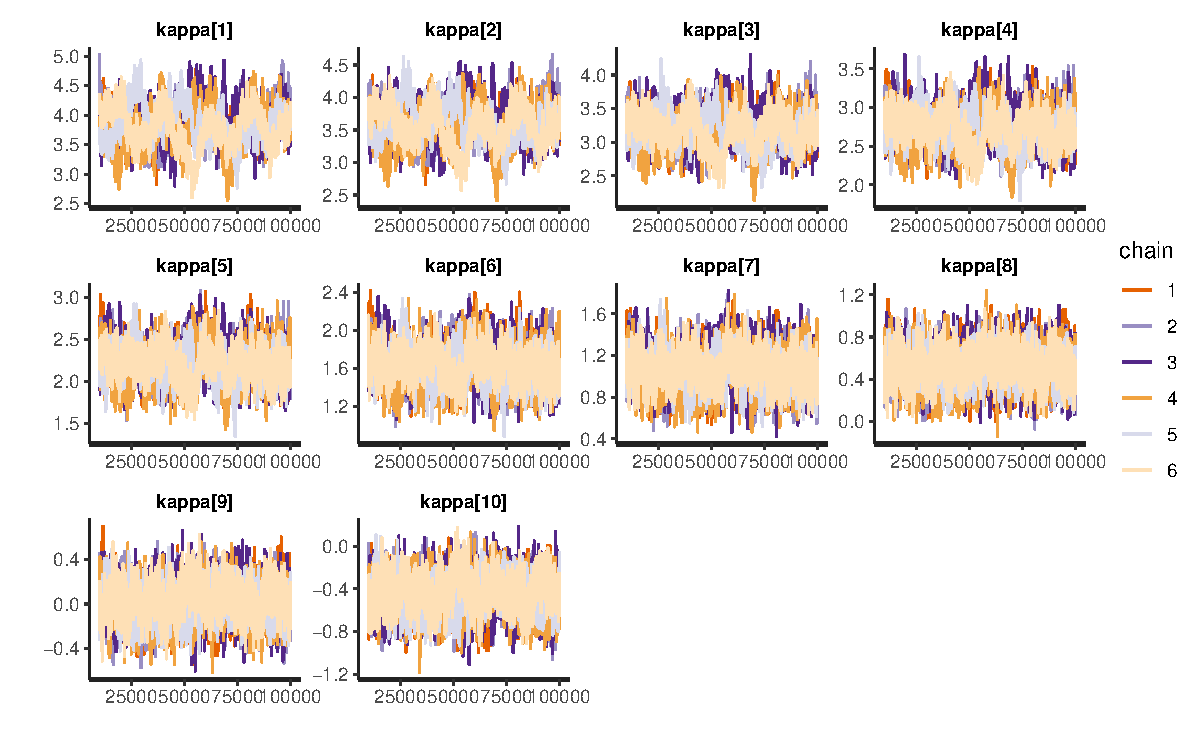
\includegraphics[width=\linewidth]{Master Thesis Code/Scripts/Synthetic data/Stan analyses/synthetic_male_stomach_lc/stan_results/trace_kappa.pdf}
        \caption{Trace plots for selected values of $\kappa_t$}
        \label{fig:synthetic_male_stomach_lc-trace-kappa}
    \end{subfigure}
    \caption{Trace plots from inference using \stan on synthetic male stomach cancer mortality. }
    \label{fig:synthetic_male_stomach_lc-trace}
\end{figure}



\newpage
\subsection{German Cancer Data}
Figures \ref{fig:obs-mr-by-age} and \ref{fig:obs-mr-by-period} displays the observed mortality rates for males and females, averaged over all years 1999-2016 and all ages 0-85+ respectively. 

% German cancer data - average over all years
\begin{figure}
    \centering
    \textbf{Mortality rates averaged over the period 1999-2016}
    \begin{subfigure}[b]{.45\linewidth}
        \includegraphics[width=\linewidth]{Master Thesis Code/Scripts/Real data/Output/Figures/observed_data/mr_stomach_by_age.pdf}
        \caption{\textbf{Stomach}: Average mortality rates for stomach cancer, male and female}
        \label{fig:obs-mr-stomach-by-age}
    \end{subfigure}
    \begin{subfigure}[b]{.45\linewidth}
        \includegraphics[width=\linewidth]{Master Thesis Code/Scripts/Real data/Output/Figures/observed_data/mr_lung_by_age.pdf}
        \caption{\textbf{Lung}: Average mortality rates for lung cancer, male and female}
        \label{fig:obs-mr-lung-by-age}
    \end{subfigure}
    \caption{Mortality rates averaged over all years, for male and females}
    \label{fig:obs-mr-by-age}
\end{figure}

% German cancer data - average over all ages
\begin{figure}
    \centering
    \textbf{Mortality rates averaged over ages 0-85+}
    \begin{subfigure}[b]{.45\linewidth}
        \includegraphics[width=\linewidth]{Master Thesis Code/Scripts/Real data/Output/Figures/observed_data/mr_stomach_by_period.pdf}
        \caption{\textbf{Stomach}: Average mortality rates for stomach cancer, male and female}
        \label{fig:obs-mr-stomach-by-period}
    \end{subfigure}
    \begin{subfigure}[b]{.45\linewidth}
        \includegraphics[width=\linewidth]{Master Thesis Code/Scripts/Real data/Output/Figures/observed_data/mr_lung_by_period.pdf}
        \caption{\textbf{Lung}: Average mortality rates for lung cancer, male and female}
        \label{fig:obs-mr-lung-by-period}
    \end{subfigure}
    \caption{Mortality rates averaged over all age groups, for male and females}
    \label{fig:obs-mr-by-period}
\end{figure}

\newpage
\subsection{Applying $\texttt{inlabru}$ to German Cancer Data}
\label{sec:real-data}

In this second part of our analysis, we will apply the previously described approach for Bayesian analysis with the Lee-Carter (LC) and the cohort-extended Lee-Carter (LCC) model to cancer data. We will use data of German mortality of lung and stomach cancer data for the years 1999-2000. 

Firstly, we apply the LC-model to the observed lung and stomach cancer mortality rates. In this step, we compare the inference results produced by \inlabru to equivalent inference results produced by \stan. We see from the plots of the observed data in Figures \ref{fig:obs-mr-by-age} and \ref{fig:obs-mr-by-period}, that the development over time of male and female cancer mortality is quite different. Therefore, it seems reasonable to treat male and female mortality separately in our model (REFER TO MULTIVARIATE STUDY SAYING NO COMMON EFFECTS GIVE THE BEST FIT?)

% Female lung - mortality rate
\begin{figure}
    \centering
    \textbf{Female lung cancer: Estimated mortality rate - LC}
    \begin{subfigure}[b]{.85\linewidth}
        \includegraphics[width=\linewidth]{Master Thesis Code/Scripts/Real data/Output/Figures/lung_rw2_lc/female/eta_x_compared.pdf}
        \caption{The mortality rate displayed as a function of calendar year, for each age group. }
        \label{fig:eta-female_lung_lc-x}
    \end{subfigure}
    
    \begin{subfigure}[b]{.85\linewidth}
        \includegraphics[width=\linewidth]{Master Thesis Code/Scripts/Real data/Output/Figures/lung_rw2_lc/female/eta_t_compared.pdf}
        \caption{The mortality rate displayed as a function of age, for each available calendar year. }
        \label{fig:eta-female_lung_lc-t}
    \end{subfigure}
    \caption{The mortality estimated by \inlabru and \stan for female lung cancer.}
    \label{fig:eta-female_lung_lc}
\end{figure}

% Female lung - random effects
\begin{figure}
    \centering
    \textbf{Female lung cancer: Estimated random effects - LC}
    \begin{subfigure}[b]{.85\linewidth}
        \includegraphics[width=\linewidth]{Master Thesis Code/Scripts/Real data/Output/Figures/lung_rw2_lc/female/random_effects_compared.pdf}
        \caption{Estimated random effects.}
        \label{fig:random-effects-female_lung_lc-re}
    \end{subfigure}
    
    \begin{subfigure}[b]{.85\linewidth}
        \includegraphics[width=\linewidth]{Master Thesis Code/Scripts/Real data/Output/Figures/lung_rw2_lc/female/hypers_compared.pdf}
        \caption{Estimated hyperparameters}
        \label{fig:random-effects-female_lung_lc-hyper}
    \end{subfigure}
    \caption{The age and period effects as estimated by \inlabru and \stan, for female lung cancer mortality. }
    \label{fig:random-effects-female_lung_lc}
\end{figure}

% Female lung - trace plots
\begin{figure}
    \centering
    \textbf{Female lung cancer: Trace plots from \stan}
    \begin{subfigure}[b]{.45\linewidth}
        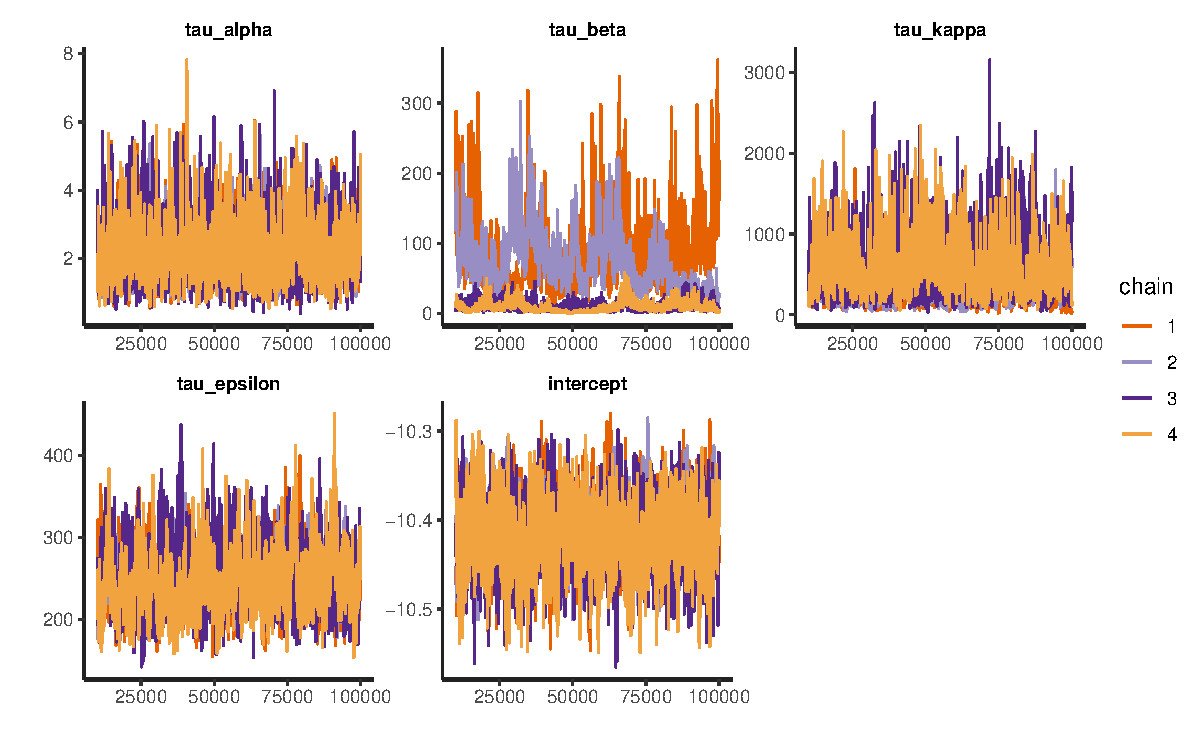
\includegraphics[width=\linewidth]{Master Thesis Code/Scripts/Real data/Stan analyses/lung_rw2_lc_female/stan_results/trace_hyperpars.pdf}
        \caption{Trace plots for hyperparameters}
        \label{fig:female-lung-lc-trace-hypers}
    \end{subfigure}
    \begin{subfigure}[b]{.45\linewidth}
        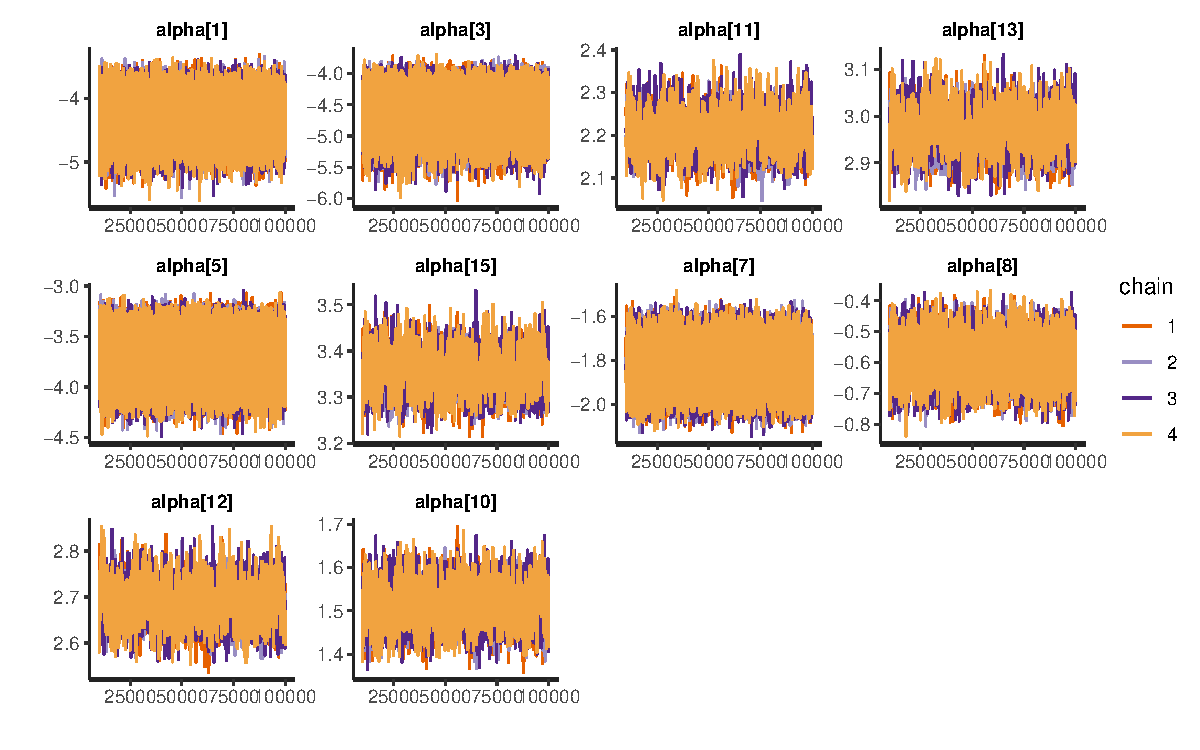
\includegraphics[width=\linewidth]{Master Thesis Code/Scripts/Real data/Stan analyses/lung_rw2_lc_female/stan_results/trace_alpha.pdf}
        \caption{Trace plots for selected values of $\alpha_x$}
        \label{fig:female-lung-lc-trace-alpha}
    \end{subfigure}
    
    \begin{subfigure}[b]{.45\linewidth}
        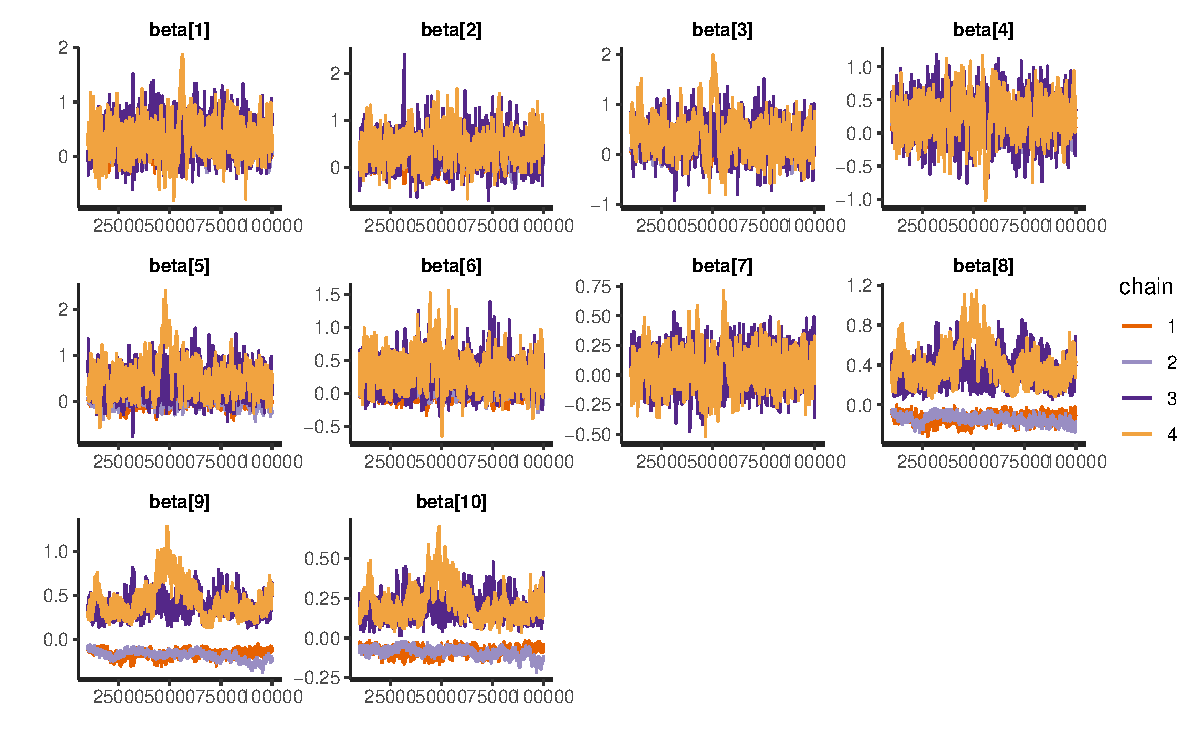
\includegraphics[width=\linewidth]{Master Thesis Code/Scripts/Real data/Stan analyses/lung_rw2_lc_female/stan_results/trace_beta.pdf}
        \caption{Trace plots for selected values of $\beta_x$}
        \label{fig:female-lung-lc-trace-beta}
    \end{subfigure}
    \begin{subfigure}[b]{.45\linewidth}
        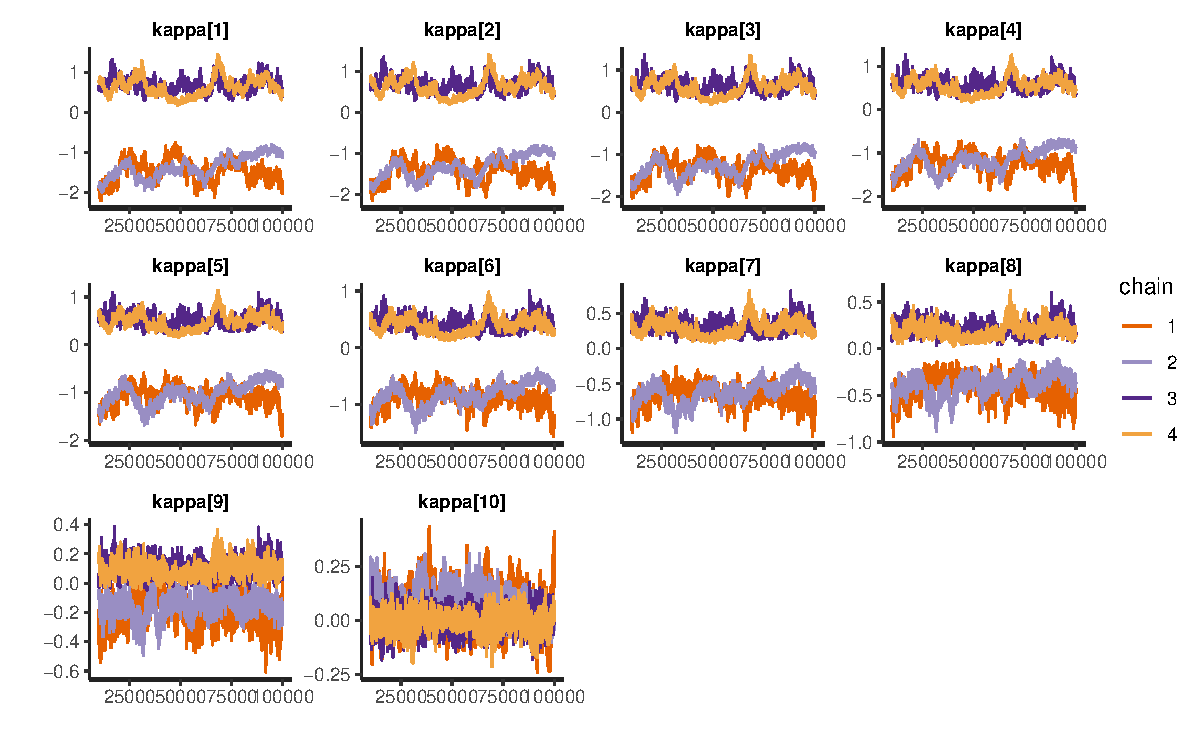
\includegraphics[width=\linewidth]{Master Thesis Code/Scripts/Real data/Stan analyses/lung_rw2_lc_female/stan_results/trace_kappa.pdf}
        \caption{Trace plots for selected values of $\kappa_t$}
        \label{fig:female-lung-lc-trace-kappa}
    \end{subfigure}
    \caption{Trace plots from inference using \stan on female lung cancer mortality. }
    \label{fig:female-lung-lc-trace}
\end{figure}

% Male lung - mortality rate
\begin{figure}
    \centering
    \textbf{Male lung cancer: Estimated mortality rate - LC}
    \begin{subfigure}[b]{.85\linewidth}
        \includegraphics[width=\linewidth]{Master Thesis Code/Scripts/Real data/Output/Figures/lung_rw2_lc/male/eta_x_compared.pdf}
        \caption{The mortality rate displayed as a function of calendar year, for each age group. }
        \label{fig:eta-male_lung_lc-x}
    \end{subfigure}
    
    \begin{subfigure}[b]{.85\linewidth}
        \includegraphics[width=\linewidth]{Master Thesis Code/Scripts/Real data/Output/Figures/lung_rw2_lc/male/eta_t_compared.pdf}
        \caption{The mortality rate displayed as a function of age, for each available calendar year. }
        \label{fig:eta-female_lung_lc-t}
    \end{subfigure}
    \caption{The mortality estimated by \inlabru and \stan for male lung cancer.}
    \label{fig:eta-male_lung_lc}
\end{figure}

% Male lung - random effects 
\begin{figure}
    \centering
    \textbf{Male lung cancer: Estimated random effects - LC}
    \begin{subfigure}[b]{.85\linewidth}
        \includegraphics[width=\linewidth]{Master Thesis Code/Scripts/Real data/Output/Figures/lung_rw2_lc/male/random_effects_compared.pdf}
        \caption{Estimated random effects.}
        \label{fig:random-effects-male_lung_lc-re}
    \end{subfigure}
    
    \begin{subfigure}[b]{.85\linewidth}
        \includegraphics[width=\linewidth]{Master Thesis Code/Scripts/Real data/Output/Figures/lung_rw2_lc/male/hypers_compared.pdf}
        \caption{Estimated hyperparameters}
        \label{fig:random-effects-male_lung_lc-hyper}
    \end{subfigure}
    \caption{The age and period effects as estimated by \inlabru and \stan, for male lung cancer mortality. }
    \label{fig:random-effects-male_lung_lc}
\end{figure}

% Male lung - trace plots
% Unavailable, weirdly saved. 

% Female stomach - mortality rate
\begin{figure}
    \centering
    \textbf{Female stomach cancer: Estimated mortality rate - LC}
    \begin{subfigure}[b]{.85\linewidth}
        \includegraphics[width=\linewidth]{Master Thesis Code/Scripts/Real data/Output/Figures/stomach_rw2_lc/female/eta_x_compared.pdf}
        \caption{The mortality rate displayed as a function of calendar year, for each age group. }
        \label{fig:eta-female_stomach_lc-x}
    \end{subfigure}
    
    \begin{subfigure}[b]{.85\linewidth}
        \includegraphics[width=\linewidth]{Master Thesis Code/Scripts/Real data/Output/Figures/stomach_rw2_lc/female/eta_t_compared.pdf}
        \caption{The mortality rate displayed as a function of age, for each available calendar year. }
        \label{fig:eta-female_stomach_lc-t}
    \end{subfigure}
    \caption{The mortality estimated by \inlabru and \stan for female stomach cancer.}
    \label{fig:eta-female_stomach_lc}
\end{figure}

% Female stomach - random effects
\begin{figure}
    \centering
    \textbf{Female stomach cancer: Estimated random effects - LC}
    \begin{subfigure}[b]{.85\linewidth}
        \includegraphics[width=\linewidth]{Master Thesis Code/Scripts/Real data/Output/Figures/stomach_rw2_lc/female/random_effects_compared.pdf}
        \caption{Estimated random effects.}
        \label{fig:random-effects-female_stomach_lc-re}
    \end{subfigure}
    
    \begin{subfigure}[b]{.85\linewidth}
        \includegraphics[width=\linewidth]{Master Thesis Code/Scripts/Real data/Output/Figures/stomach_rw2_lc/female/hypers_compared.pdf}
        \caption{Estimated hyperparameters}
        \label{fig:random-effects-female_stomach_lc-hyper}
    \end{subfigure}
    \caption{The age and period effects as estimated by \inlabru and \stan for female stomach cancer mortality. }
    \label{fig:random-effects-female_stomach_lc}
\end{figure}

% Female stomach - trace plots
\begin{figure}
    \centering
    \textbf{Female stomach cancer: Trace plots from \stan}
    \begin{subfigure}[b]{.45\linewidth}
        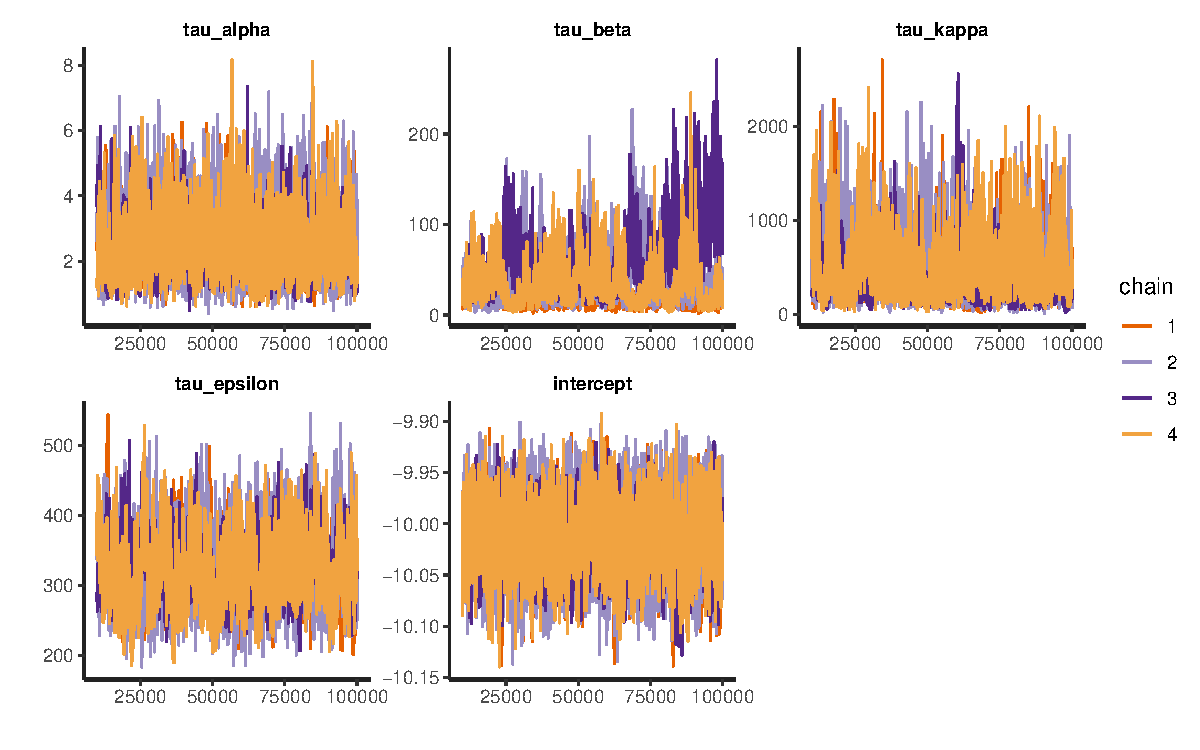
\includegraphics[width=\linewidth]{Master Thesis Code/Scripts/Real data/Stan analyses/stomach_rw2_lc_female/stan_results/trace_hyperpars.pdf}
        \caption{Trace plots for hyperparameters}
        \label{fig:female-stomach-lc-trace-hypers}
    \end{subfigure}
    \begin{subfigure}[b]{.45\linewidth}
        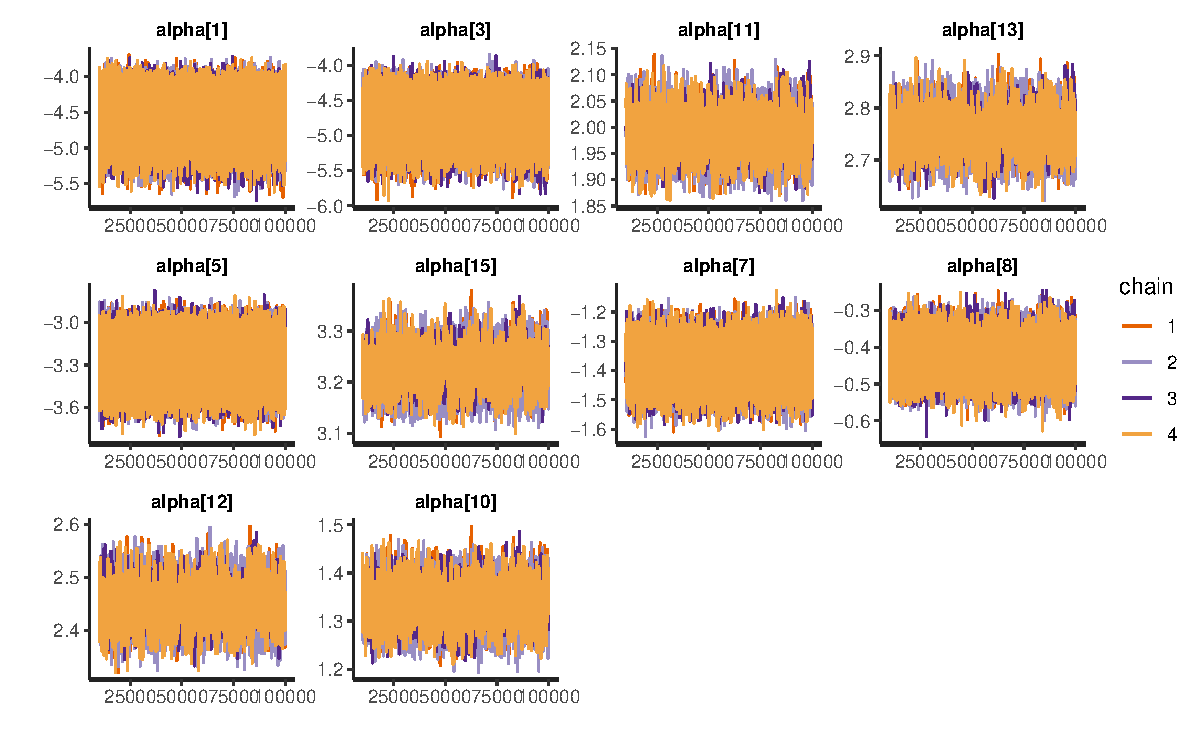
\includegraphics[width=\linewidth]{Master Thesis Code/Scripts/Real data/Stan analyses/stomach_rw2_lc_female/stan_results/trace_alpha.pdf}
        \caption{Trace plots for selected values of $\alpha_x$}
        \label{fig:female-stomach-lc-trace-alpha}
    \end{subfigure}
    
    \begin{subfigure}[b]{.45\linewidth}
        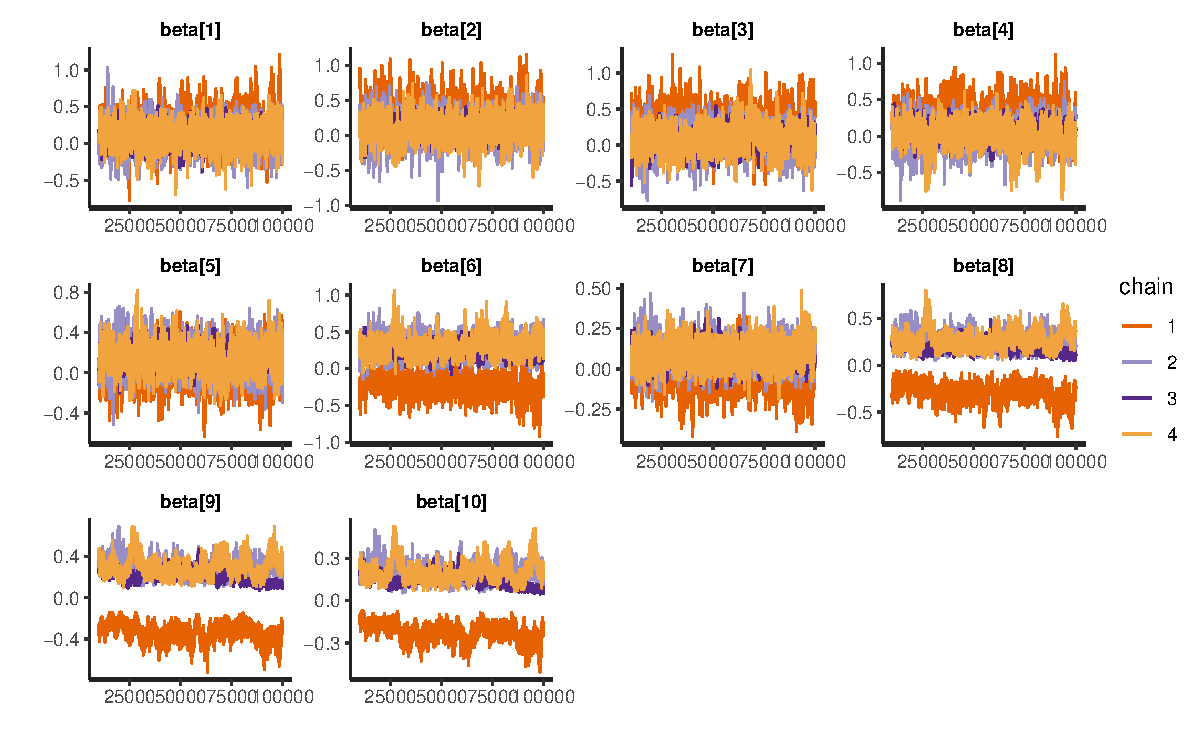
\includegraphics[width=\linewidth]{Master Thesis Code/Scripts/Real data/Stan analyses/stomach_rw2_lc_female/stan_results/trace_beta.pdf}
        \caption{Trace plots for selected values of $\beta_x$}
        \label{fig:female-stomach-lc-trace-beta}
    \end{subfigure}
    \begin{subfigure}[b]{.45\linewidth}
        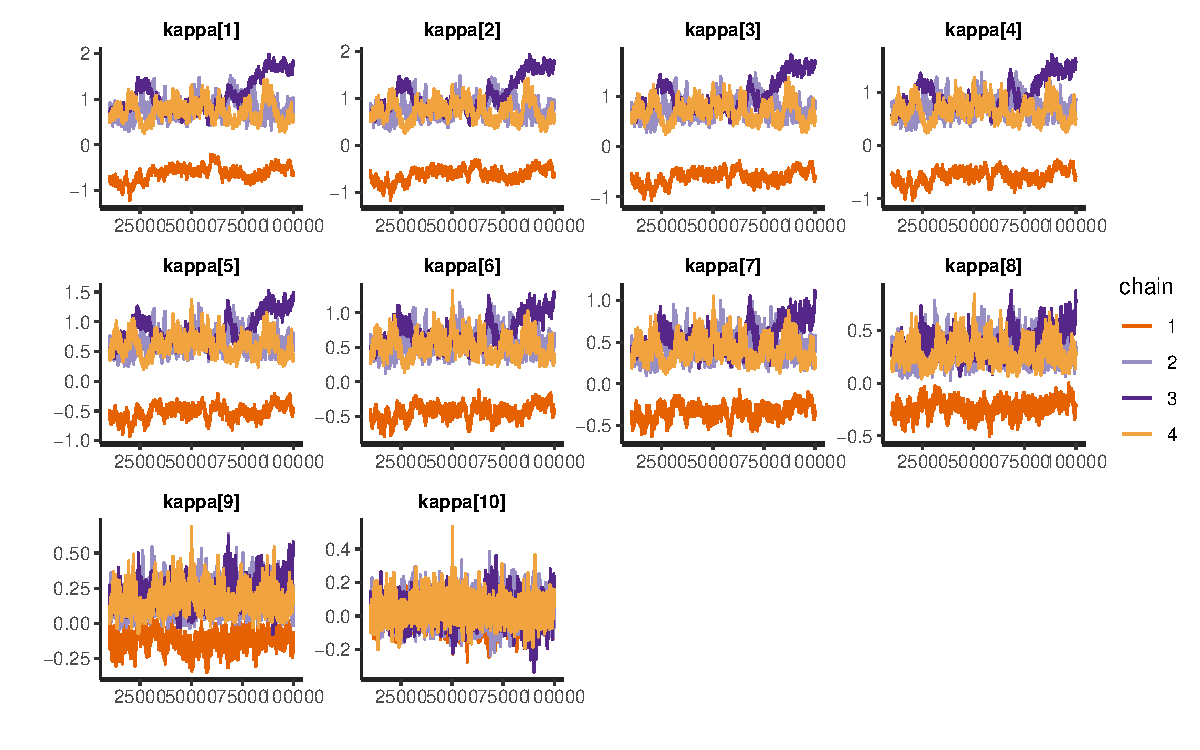
\includegraphics[width=\linewidth]{Master Thesis Code/Scripts/Real data/Stan analyses/stomach_rw2_lc_female/stan_results/trace_kappa.pdf}
        \caption{Trace plots for selected values of $\kappa_t$}
        \label{fig:female-stomach-lc-trace-kappa}
    \end{subfigure}
    \caption{Trace plots from inference using \stan on female stomach cancer mortality. }
    \label{fig:female-stomach-lc-trace}
\end{figure}

% Male stomach - mortality rate
\begin{figure}
    \centering
    \textbf{Male stomach cancer: Estimated mortality rate - LC}
    \begin{subfigure}[b]{.85\linewidth}
        \includegraphics[width=\linewidth]{Master Thesis Code/Scripts/Real data/Output/Figures/stomach_rw2_lc/male/eta_x_compared.pdf}
        \caption{The mortality rate displayed as a function of calendar year, for each age group. }
        \label{fig:eta-male_stomach_lc-x}
    \end{subfigure}
    
    \begin{subfigure}[b]{.85\linewidth}
        \includegraphics[width=\linewidth]{Master Thesis Code/Scripts/Real data/Output/Figures/stomach_rw2_lc/male/eta_t_compared.pdf}
        \caption{The mortality rate displayed as a function of age, for each available calendar year. }
        \label{fig:eta-male_stomach_lc-t}
    \end{subfigure}
    \caption{The mortality estimated by \inlabru and \stan for male stomach cancer.}
    \label{fig:eta-male_stomach_lc}
\end{figure}

% Male stomach - random effects
\begin{figure}
    \centering
    \textbf{Male stomach cancer: Estimated random effects - LC}
    \begin{subfigure}[b]{.85\linewidth}
        \includegraphics[width=\linewidth]{Master Thesis Code/Scripts/Real data/Output/Figures/stomach_rw2_lc/male/random_effects_compared.pdf}
        \caption{Estimated random effects.}
        \label{fig:random-effects-male_stomach_lc-re}
    \end{subfigure}
    
    \begin{subfigure}[b]{.85\linewidth}
        \includegraphics[width=\linewidth]{Master Thesis Code/Scripts/Real data/Output/Figures/stomach_rw2_lc/male/hypers_compared.pdf}
        \caption{Estimated hyperparameters}
        \label{fig:random-effects-male_stomach_lc-hyper}
    \end{subfigure}
    \caption{The age and period effects as estimated by \inlabru and \stan for male stomach cancer mortality. }
    \label{fig:random-effects-male_stomach_lc}
\end{figure}

% Male stomach - trace plots
\begin{figure}
    \centering
    \textbf{Male stomach cancer: Trace plots from \stan}
    \begin{subfigure}[b]{.45\linewidth}
        \includegraphics[width=\linewidth]{Master Thesis Code/Scripts/Real data/Stan analyses/stomach_rw2_lc_male/stan_results/trace_hyperpars.pdf}
        \caption{Trace plots for hyperparameters}
        \label{fig:male-stomach-lc-trace-hypers}
    \end{subfigure}
    \begin{subfigure}[b]{.45\linewidth}
        \includegraphics[width=\linewidth]{Master Thesis Code/Scripts/Real data/Stan analyses/stomach_rw2_lc_male/stan_results/trace_alpha.pdf}
        \caption{Trace plots for selected values of $\alpha_x$}
        \label{fig:male-stomach-lc-trace-alpha}
    \end{subfigure}
    
    \begin{subfigure}[b]{.45\linewidth}
        \includegraphics[width=\linewidth]{Master Thesis Code/Scripts/Real data/Stan analyses/stomach_rw2_lc_male/stan_results/trace_beta.pdf}
        \caption{Trace plots for selected values of $\beta_x$}
        \label{fig:male-stomach-lc-trace-beta}
    \end{subfigure}
    \begin{subfigure}[b]{.45\linewidth}
        \includegraphics[width=\linewidth]{Master Thesis Code/Scripts/Real data/Stan analyses/stomach_rw2_lc_male/stan_results/trace_kappa.pdf}
        \caption{Trace plots for selected values of $\kappa_t$}
        \label{fig:male-stomach-lc-trace-kappa}
    \end{subfigure}
    \caption{Trace plots from inference using \stan on male stomach cancer mortality. }
    \label{fig:male-stomach-lc-trace}
\end{figure}



Figures \ref{fig:mr-lcc-stomach} and \ref{fig:random-effects-lcc-stomach} displays the stomach cancer mortality rates and age, period and cohort effects, with their associated hyperparameters, as estimated by $\texttt{inlabru}$ for the LCC-model. These results are produced in the script \url{Master Thesis Code/Scripts/Real data/run_inlabru_real_data.R}.

\begin{figure}
    \centering
    \textbf{LCC-model: estimated mortality rates for stomach cancer}
    \begin{subfigure}[b]{.45\linewidth}
        \includegraphics[width=\linewidth]{Master Thesis Code/Scripts/Real data/Output/Figures/stomach_rw2/mr_x_inlabru.pdf}
        \caption{Mortality rates displayed as a function of calendar year, for each age group. }
        \label{fig:mr-lcc-stomach-x}
    \end{subfigure}
    \begin{subfigure}[b]{.45\linewidth}
        \includegraphics[width=\linewidth]{Master Thesis Code/Scripts/Real data/Output/Figures/stomach_rw2/mr_t_inlabru.pdf}
        \caption{The mortality rates displayed as a function of age, for each available calendar year. }
        \label{fig:mr-lcc-stomach-t}
    \end{subfigure}
    \caption{The stomach cancer mortality rate estimated by $\texttt{inlabru}$ displayed together with the observed stomach cancer mortality rate.}
    \label{fig:mr-lcc-stomach}
\end{figure}

\begin{figure}
    \centering
    \textbf{LCC-model: estimated age, period and cohort effects for stomach cancer}
    \begin{subfigure}[b]{.85\linewidth}
        \includegraphics[width=\linewidth]{Master Thesis Code/Scripts/Real data/Output/Figures/stomach_rw2/random_effects_inlabru.pdf}
        \caption{Estimated random effects.}
        \label{fig:random-effects-lcc-stomach-re}
    \end{subfigure}
    
    \begin{subfigure}[b]{.85\linewidth}
        \includegraphics[width=\linewidth]{Master Thesis Code/Scripts/Real data/Output/Figures/stomach_rw2/hypers_inlabru.pdf}
        \caption{Estimated hyperparameters}
        \label{fig:random-effects-lcc-stomach-hyper}
    \end{subfigure}
    \caption{The random age- period and cohort effects, as well as the hyperparameters, estimated by applying the LCC-model to stomach cancer mortality data by $\texttt{inlabru}$.}
    \label{fig:random-effects-lcc-stomach}
\end{figure}

Figures \ref{fig:mr-lcc-lung} and \ref{fig:random-effects-lcc-lung} displays the lung cancer mortality rates and age, period and cohort effects, with their associated hyperparameters, as estimated by $\texttt{inlabru}$ for the LDD-model. These results are produced in the script \url{Master Thesis Code/Scripts/Real data/run_inlabru_real_data.R}.

\begin{figure}
    \centering
    \textbf{LCC-model: estimated mortality rates for lung cancer}
    \begin{subfigure}[b]{.45\linewidth}
        \includegraphics[width=\linewidth]{Master Thesis Code/Scripts/Real data/Output/Figures/lung_rw2/mr_x_inlabru.pdf}
        \caption{Mortality rates displayed as a function of calendar year, for each age group. }
        \label{fig:mr-lcc-lung-x}
    \end{subfigure}
    \begin{subfigure}[b]{.45\linewidth}
        \includegraphics[width=\linewidth]{Master Thesis Code/Scripts/Real data/Output/Figures/lung_rw2/mr_t_inlabru.pdf}
        \caption{The mortality rates displayed as a function of age, for each available calendar year. }
        \label{fig:mr-lcc-lung-t}
    \end{subfigure}
    \caption{The lung cancer mortality rate estimated by $\texttt{inlabru}$ displayed together with the observed lung cancer mortality rate.}
    \label{fig:mr-lcc-lung}
\end{figure}

\begin{figure}
    \centering
    \textbf{LCC-model: estimated age, period and cohort effects for lung cancer}
    \begin{subfigure}[b]{.85\linewidth}
        \includegraphics[width=\linewidth]{Master Thesis Code/Scripts/Real data/Output/Figures/lung_rw2/random_effects_inlabru.pdf}
        \caption{Estimated random effects.}
        \label{fig:random-effects-lcc-lung-re}
    \end{subfigure}
    
    \begin{subfigure}[b]{.85\linewidth}
        \includegraphics[width=\linewidth]{Master Thesis Code/Scripts/Real data/Output/Figures/lung_rw2/hypers_inlabru.pdf}
        \caption{Estimated hyperparameters}
        \label{fig:random-effects-lcc-lung-hyper}
    \end{subfigure}
    \caption{The age- period and cohort effects, as well as the hyperparameters, estimated by applying the LCC-model to lung cancer mortality data by $\texttt{inlabru}$.}
    \label{fig:random-effects-lcc-lung}
\end{figure}

\newpage
\subsection{Using LCC-model for Prediction}

Figures \ref{fig:mr-pred-stomach} and \ref{fig:random-effects-pred-stomach} displays the results of applying the LCC-model to German stomach cancer mortality data. The observed mortality rates for years 1999-2007 are used to predict the mortality rates, and the associated age, period and cohort effects, for the years 2008-2016. These results are produced in the script \url{Master Thesis Code/Scripts/Real data/run_inlabru_real_data.R}.

\begin{figure}
    \centering
    \textbf{Prediction with LCC-model for stomach cancer mortality}
    \begin{subfigure}[b]{.85\linewidth}
        \includegraphics[width=\linewidth]{Master Thesis Code/Scripts/Real data/Output/Figures/stomach_rw2_predict/mr_x_inlabru.pdf}
        \caption{Mortality rates displayed as a function of calendar year, for each age group. }
        \label{fig:mr-pred-stomach-x}
    \end{subfigure}
    
    \begin{subfigure}[b]{.85\linewidth}
        \includegraphics[width=\linewidth]{Master Thesis Code/Scripts/Real data/Output/Figures/stomach_rw2_predict/mr_t_inlabru.pdf}
        \caption{The mortality rates displayed as a function of age, for each available calendar year. }
        \label{fig:mr-pred-stomach-t}
    \end{subfigure}
    \caption{The stomach cancer mortality rate estimated and predicted by $\texttt{inlabru}$ displayed together with the observed stomach cancer mortality rate. The predicted mortality rates are marked with blue triangles, while the estimated mortality rates for which we have observed data are marked with blue crosses.}
    \label{fig:mr-pred-stomach}
\end{figure}

\begin{figure}
    \centering
    \textbf{Estimated and predicted age, period and cohort effects with LCC-model for stomach cancer mortality}
    \begin{subfigure}[b]{.85\linewidth}
        \includegraphics[width=\linewidth]{Master Thesis Code/Scripts/Real data/Output/Figures/stomach_rw2_predict/random_effects_inlabru.pdf}
        \caption{Estimated random effects. The estimates for the period effect $\kappa_t$ for the unobserved years are marked with yellow triangles. The estimates for the cohort effect $\gamma_c$ for the partially observed and unobserved cohorts are marked with green crosses and yellow triangles, respectively. }
        \label{fig:random-effects-pred-stomach-re}
    \end{subfigure}
    
    \begin{subfigure}[b]{.85\linewidth}
        \includegraphics[width=\linewidth]{Master Thesis Code/Scripts/Real data/Output/Figures/stomach_rw2_predict/hypers_inlabru.pdf}
        \caption{Estimated hyperparameters}
        \label{fig:random-effects-pred-stomach-hyper}
    \end{subfigure}
    \caption{The random age- period and cohort effects, as well as the hyperparameters, estimated by applying the LCC-model to stomach cancer mortality data by $\texttt{inlabru}$.}
    \label{fig:random-effects-pred-stomach}
\end{figure}

Figures \ref{fig:mr-pred-lung} and \ref{fig:random-effects-pred-lung} displays the results of applying the LCC-model to German stomach cancer mortality data. The observed mortality rates for years 1999-2007 are used to predict the mortality rates, and the associated age, period and cohort effects, for the years 2008-2016. 


\begin{figure}
    \centering
    \begin{subfigure}[b]{.85\linewidth}
        \includegraphics[width=\linewidth]{Master Thesis Code/Scripts/Real data/Output/Figures/lung_rw2_predict/mr_x_inlabru.pdf}
        \caption{Mortality rates displayed as a function of calendar year, for each age group. }
        \label{fig:mr-pred-lung-x}
    \end{subfigure}
    
    \begin{subfigure}[b]{.85\linewidth}
        \includegraphics[width=\linewidth]{Master Thesis Code/Scripts/Real data/Output/Figures/lung_rw2_predict/mr_t_inlabru.pdf}
        \caption{The mortality rates displayed as a function of age, for each available calendar year. }
        \label{fig:mr-pred-lung-t}
    \end{subfigure}
    \caption{The lung cancer mortality rate estimated and predicted by $\texttt{inlabru}$ displayed together with the observed lung cancer mortality rate. The predicted mortality rates are marked with blue triangles, while the estimated mortality rates for which we have observed data are marked with blue crosses.}
    \label{fig:mr-pred-lung}
\end{figure}

\begin{figure}
    \centering
    \begin{subfigure}[b]{.85\linewidth}
        \includegraphics[width=\linewidth]{Master Thesis Code/Scripts/Real data/Output/Figures/lung_rw2_predict/random_effects_inlabru.pdf}
        \caption{Estimated random effects. The estimates for the period effect $\kappa_t$ for the unobserved years are marked with yellow triangles. The estimates for the cohort effect $\gamma_c$ for the partially observed and unobserved cohorts are marked with green crosses and yellow triangles, respectively. }
        \label{fig:random-effects-pred-lung-re}
    \end{subfigure}
    
    \begin{subfigure}[b]{.85\linewidth}
        \includegraphics[width=\linewidth]{Master Thesis Code/Scripts/Real data/Output/Figures/lung_rw2_predict/hypers_inlabru.pdf}
        \caption{Estimated hyperparameters}
        \label{fig:random-effects-pred-lung-hyper}
    \end{subfigure}
    \caption{The random age- period and cohort effects, as well as the hyperparameters, estimated by applying the LCC-model to lung cancer mortality data by $\texttt{inlabru}$.}
    \label{fig:random-effects-pred-lung}
\end{figure}

